\section{Consultar Pacientes}

Un doctor contará con la facultad de consultar los pacientes de los que son o fueron responsables de sus tratamientos y así poder tener un conocimiento de éstos.

\subsubsection{Procedimiento}
\begin{enumerate}
	
	\item Da clic en el icono \textbf{Pacientes} de la pantalla \textbf{Menú Principal del Doctor}.

		\begin{figure}[!htbp]			\hypertarget{fig:mpDoctor2}{\hspace{1pt}}
		\begin{center}
			\includegraphics[height=0.4\textheight]{images/Iconos/Advertencia}
			\caption{Menú Principal del Doctor}
			\label{fig:mpDoctor2}
		\end{center}
	\end{figure}

	\item Se mostrará la pantalla \textbf{Pacientes}. 
	\newpage
	\begin{figure}[!htbp]			
		\hypertarget{fig:Pacientes}{\hspace{1pt}}
		\begin{center}
			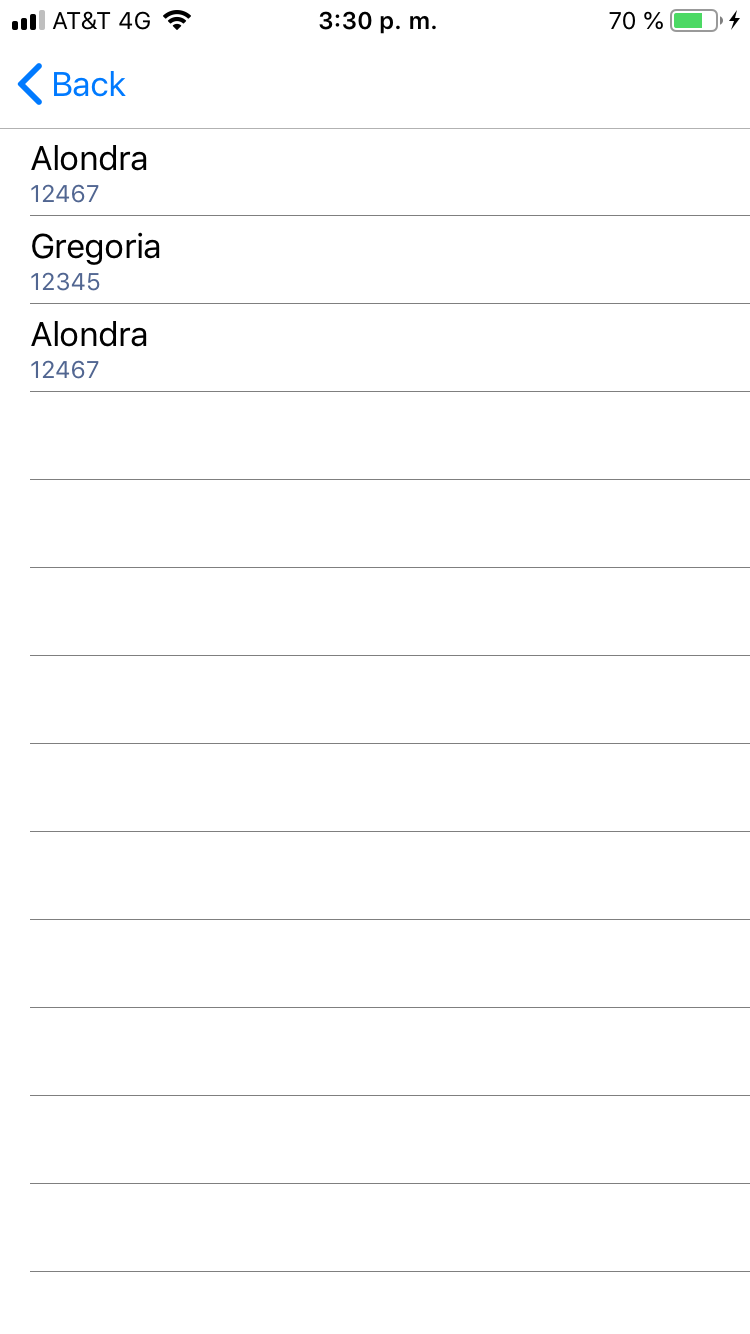
\includegraphics[height=0.4\textheight]{Doctor/ConsultarPacientes/images/Pacientes}
			\caption{Pacientes}
			\label{fig:Pacientes}
		\end{center}
	\end{figure}

	
\end{enumerate}

